\chapter{Introduction and Context}
\label{Chapter1}

\section{Introduction}
Technology's world is evolving very fast. Every year new tools, frameworks\footnote{A software framework is an abstraction in which software providing generic functionality can be selectively changed by additional user-written code, thus providing application-specific software. \href{https://en.wikipedia.org/wiki/Software_framework}{Wikipedia}} programming languages, etc. are released. Some of them are living they gold's era, such as blockchain and machine learning,  while others are forgotten.  

This makes hard for universities decide what to teach: the tools used by companies or the fundaments of informatics.  

This project works with the fundaments of informatics and logic which won't change either be forgotten.  


In this project, we will work with Pseudo-Boolean Minimization widely used by a lot of technologies such as Artifical Intelligence, Planners, Computer Vision,  Circuit design, ... 

%TODO: Appendix with an example

\section{Context} 


But before being able to explain the main problem which this project is about, Pseudo-Boolean Minimization, it necessary to do a quick introduction to a much wider topic. 


Boolean satisfiability problems (SAT from now on) is the problem of finding a model for a Boolean Formula (BF from now on). In other words, it is the result of evaluating the BF after replacing its variables for true or false. 

SAT is widely used in Computer Science because it was the first problem proved to be NP-Complete which allowed a lot of NP problems be reduced to it\cite{Cook1971}

\subsection{What is a Pseudo-Boolean Formula?}
In propositional logic, a \emph{BF} is defined as following\cite{Lpo}:\\
Let $P$ be a set of predicate symbols like $p,q,r,...$
\begin{itemize}
	\item All predicate symbol of $P$ is a formula.
	\item If $F$ and $G$ are formulae, then $(F \land G)$ and $(F \lor G)$ are formulae too.
	\item If $F$ is a formula, then $(\neg F)$ is a formula.
	\item Nothing else is a formula.
\end{itemize}
This representation has some limitations because it can only express properties which are \emph{true} or \emph{false}.\\

%TODO: Example of boolean formula: variables, predicate symbols, interpretations, models, etc...

\subsection{What are pseudo-boolean formulae?}

\emph{Pseudo-Boolean Formulas} are functions of the form $f:B^n \rightarrow \mathbb{R}$. For example, the following formula is a \emph{Pseudo-Boolean Formula} (PBF from now on): $3x+5y$. Therefore, \emph{BF} are a special case of \emph{PBF} where the domain is $d=\{0,1\}$.\\

%TODO: potser explicar que son cardinality constraints


\subsection{Pseudo-Boolean minimization}
Pseudo-boolean optimizations is a linear programming problem: \\\\
\noindent\makebox[\linewidth]{\rule{\linewidth}{0.4pt}}
Linear programming (LP, also called linear optimization) is a method to achieve the best
outcome (such as maximum profit or lowest cost) in a mathematical model whose requirements
are represented by linear relationships. 

Linear programs are problems that can be expressed in canonical formas

\begin{center}
	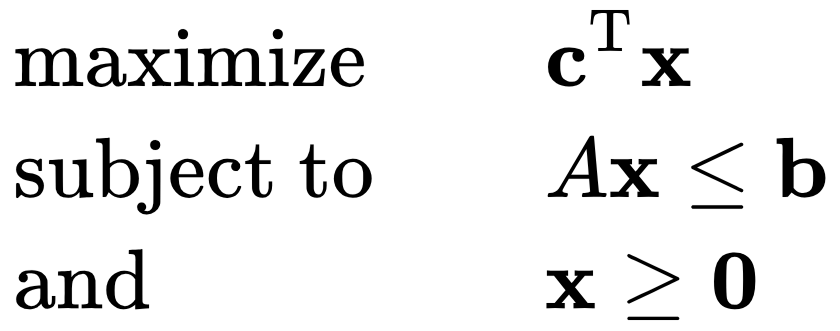
\includegraphics[width=0.3\textwidth]{Figures/linearProgramming.png}
	\captionof{figure}{Linear programming canonical form representation}
\end{center}

where x represents the vector of variables (to be determined), c and bare vectors of (known)
coefficients, A is a (known) matrix of coefficients, and is the matrix transpose. The expression to be maximized or minimized is called the objective function (c Tx in this case). The inequalities Ax $\leq$ b and x $\geq$ 0 are the constraints which specify a convex polytope over which the
objective function is to be optimized.
\begin{center}
	\href{https://en.wikipedia.org/wiki/Linear\_programming}{https://en.wikipedia.org/wiki/Linear\_programming}
\end{center}
\noindent\makebox[\linewidth]{\rule{\linewidth}{0.4pt}}


Pseudo-boolean minimization is a particular case where the objective function (also called) cost function is minimized, the variables are boolean {0,1} and the variable’s coefficients are integers.  

In other words, a pseudo-boolean minimization problem has two components: 
\begin{itemize}
	\item A set of pseudo-boolean constraints \\
	of the form $\sum_{i=1}^{n} x_{i}w_{i} \leq k$, where $w_{i},k \in \mathbb{I}$ and $x_{i} \in \{0,1\}$
	\item A cost function
\end{itemize}


%TODO: Example of the two things



The goal is to minimize the cost function $min(a_{1}x{1} + ... + a_{n}x_{n})$. Find an assignment for the problem’s variables in a way that all the constraints are satisfied and the evaluation of the cost function is minimum.  

The value m is minimum, if m-1 is unsatisfiable.  



%TODO: Example of pseudo-boolean minimization problem, variables, constraints, cost function and solutions. Also optimal solution) 



There is a big research in this field, more specifically in encoding PBF into CNF. In this paper, Hölldobler, Manthey, Steinke\cite{Holldobler}, some relevant PBF into SAT encodings are explained and a new one is proposed. One of the authors of this paper, Steinke, is also the author of PBLib. 
 

\section{Background}

During the past semester (Q1 2017/2018), under the supervision of \href{https://www.cs.upc.edu/~jordicf/}{Dr. Jordi Cortadella}, I had been developing a C++ library.\\
This tool allows the users to represent \emph{BF} in a C++ program in an intuitive way, do operations between them and convert them into \emph{Binary Decision Diagrams} (BDD from now on). However, the main functionality of this library is the conversion from a \emph{BF} to \emph{CNF}.  \\
As previously explained, \emph{CNF} is a particular type of a \emph{BF}, a conjunction of disjunctions. \emph{CNF} is an important format because it is the standard input for \emph{SAT Solvers}\ref{A.1}.\\
As shown in this paper, \emph{Mitchell, Selman, and Levesque\cite{Mitchell}}, there is a correlation between the number of variables, the number of clauses and the hardness of solving the \emph{CNF}.
\begin{center}
	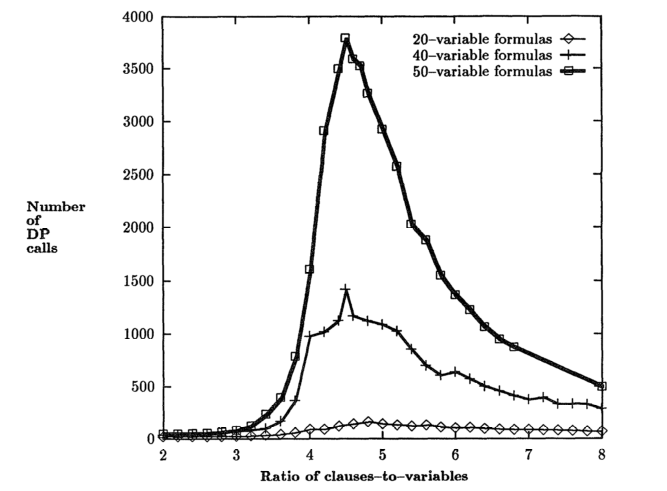
\includegraphics[width=1\textwidth]{Figures/GraphMitchellSelmanLevesque.png}
	\captionof{figure}{Median number of recursive DP calls for Random 3-SAT formulas, as a function of the ratio of clauses-to-variables. \\Extracted from Mitchell, Selman, and Levesque\cite{Mitchell}}
\end{center}
Therefore, an improvement of the input \emph{CNF} of the \emph{SAT Solver} can reduce a lot the hardness of the problem. \\
This is the main goal of the library, try to reduce the size of the final \emph{CNF} resulting from applying different converting methods on the original BF.

\section{State-of-the-art}

%TODO: explicar encodings que hi ha per sat (que implementi PBLib per exemple)
%TODO: explicar minisat


Nowadays there is a well known C++ library called \href{http://tools.computational-logic.org/content/pblib.php}{PBLib} developed by Peter Steinke. PBLib allows its users to represent pseudo-boolean constraints and encode them into a CNF.  
It possesses a big repertory of encodings which have been proposed in the past in different papers\cite{Steinke2015}.  
\begin{center}
	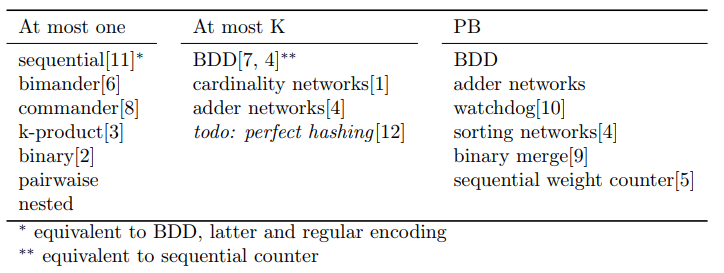
\includegraphics[width=1\textwidth]{Figures/PBLibEncodings.png}
	\captionof{figure}{PBLib implemented encodings\\Extracted from Steinke\cite{Steinke2015}}
\end{center}
Apart from having these encodings, PBLib applies the best one for the given pseudo-boolean constraint in a way that provides the most effective translation. 

In Chapter3 - Development \ref{Chapter3} PBLib is discussed as a tool for this project. In a nutshell, PBLib is a very good tool developed by professionals and it will be hard to try to do the same with the same quality. For these reasons, and some others explained in more detail in Chapter 3, PBLib has been incorporated in this project as a translator of pseudo-boolean constraints to CNF.  

One of the downsides of PBLib is the interface which is not very user-friendly. As can be seen in Chapter 2 Objectives\ref{Chapter2}, one of the objectives of this project is offering a good interface which means that a layer between the user and PBLib will be added to simplify how the users declare pseudo-boolean constraints.  

%TODO: maybe an appendix or something explaining PBlib encodings in more detail


The second project we will talk about is the explained in the \emph{Background section}. This project adds a new encoding for \emph{BF} which can be extended to \emph{PB Constraints}. This encoding will be studied and if it achieves good metrics it will be implemented to \emph{PB Constraints}


\section{Motivations}

\href{https://www.fib.upc.edu/en/studies/bachelors-degrees/bachelor-degree-informatics-engineering/curriculum/syllabus/LI}{Informatics Logic} is taught in this\footnote{\href{https://www.fib.upc.edu/en/}{Facultat Informàtica de Barcelona}} faculty. In that course, I realized how important is \emph{logic} through its lecturer, \href{http://www.lsi.upc.es/~roberto/}{Dr. Robert Nieuwenhuis}, and its activities. \\

In the first coursework, we had to code a \emph{SAT Solver} which used \emph{Unit Propagation}.
%\ref{A.2}. 
With this activity, I comprehended how hard and substantial is the study of \emph{logic} and all its context. For example, how \emph{logic} is used in Artificial Intelligence and Planners.\\

When the time of deciding the \emph{TFG} arrived, I contacted my actual supervisor, \href{https://www.cs.upc.edu/~jordicf/}{Dr. Jordi Cortadella}, and he proposed me some topics and ideas. Finally, we agreed on doing this project. \\

The motivation for this project is trying to deepen into the topic and contribute on it.

Also during the studies, with the transversal competencies, there has been an intention to teach students about sustainability and its importance. %TODO: if found, attach a link to some environmental talk

As previously told, the subject of this project is widely used in many other areas which have a big footprint because of electricity consumption. This is also a motivation for this project because reducing the execution time will become in a decrease of electricity spent and that will be beneficial for the climate.  

\section{Stakeholders}

In this section, the Stakeholders of the project are defined. Stakeholders are entities which are affected, directly or indirectly, by the solution developed in this project. 
\subsection{Target audience}
This tools targets all the entities (researchers, companies, \ldots) which work with \emph{PB minimization} and use \emph{SAT Solvers}.
\subsection{Users}
The users will be C++ programmers due this tool is developed in this language.
\subsection{Beneficiaries}
All those entities which work with \emph{PB minimization}. For example AI, SAT Solvers, Planners, \ldots